\documentclass[11pt]{article}
\usepackage[margin=1in]{geometry}
\usepackage{booktabs}
\usepackage{siunitx}
\usepackage{pgfplots}
\usepackage{hyperref}
\pgfplotsset{compat=1.17}
\sisetup{
  round-mode=places,
  round-precision=4
}

\title{CSC367 Project Part 1 Report\\Serial and OpenMP Particle Simulation}
\author{
  Ashish Ajin Thomas (\texttt{thoma898}) \and
  Rithvik Sunil (\texttt{sunilrit})
}
\date{March 11, 2026}

\begin{document}
\maketitle

\section{Overview}
This report documents the Part 1 implementation and measurements for the particle
simulation. The starter code's force computation is \(\mathcal{O}(n^2)\), while
our modified \texttt{serial.cpp} and \texttt{openmp.cpp} use spatial binning to
achieve expected \(\mathcal{O}(n)\) behavior at the assignment's particle density.

\section{Implementation}
\subsection{Serial (\texttt{serial.cpp})}
We partition the simulation box into a 2D grid of cells whose width is at least
\texttt{CUTOFF}. At each timestep:
\begin{enumerate}
  \item Clear cell heads.
  \item Bin particles by position into linked lists (\texttt{cellFirst}, \texttt{nextInCell}).
  \item For each particle, compute forces from particles in the local \(3\times3\) cell neighborhood only.
  \item Move particles with \texttt{move()}.
\end{enumerate}
Because expected particles per cell are bounded at fixed density, force work per
particle is expected constant, giving overall \(\mathcal{O}(n)\) time per step.

\subsection{OpenMP (\texttt{openmp.cpp})}
The same cell-list algorithm is used, with these parallelization choices:
\begin{itemize}
  \item Cell-list reset + binning are done in an OpenMP \texttt{single} region (avoids lock contention).
  \item Force loop is parallelized with \texttt{\#pragma omp for schedule(static)} and reductions.
  \item \texttt{dmin} is thread-private, then merged via a critical section.
  \item Move loop is parallelized with static scheduling.
\end{itemize}

\section{Correctness}
Correctness is checked with assignment-provided metrics:
\texttt{absmin} should remain \(> 0.4\) and \texttt{absavg} should be close to
\(\sim 0.95\). From compute-node run \texttt{part1-report\_3117.out}:
\begin{quote}
\texttt{Serial: n = 1000, simulation time = 0.094633 seconds, absmin = 0.772844, absavg = 0.957457}\\
\texttt{OpenMP: n = 5000,threads = 16, simulation time = 0.314934 seconds, absmin = 0.775466, absavg = 0.957188}
\end{quote}
Both runs satisfy \(\texttt{absmin} > 0.4\) and \(\texttt{absavg} \approx 0.95\), so
the force interactions are computed correctly.

\section{Serial Results}
\subsection{Runtime Tables}
\begin{table}[h]
\centering
\caption{Serial runtime (small set)}
\begin{tabular}{rr}
\toprule
\(n\) & time (s) \\
\midrule
500 & 0.029217 \\
1000 & 0.060744 \\
1500 & 0.092168 \\
2000 & 0.123194 \\
3000 & 0.186291 \\
4000 & 0.251289 \\
6000 & 0.380784 \\
8000 & 0.512006 \\
\bottomrule
\end{tabular}
\end{table}

\begin{table}[h]
\centering
\caption{Serial runtime (large set)}
\begin{tabular}{rr}
\toprule
\(n\) & time (s) \\
\midrule
10000 & 0.645118 \\
20000 & 1.384450 \\
40000 & 2.993740 \\
80000 & 6.510580 \\
160000 & 13.036700 \\
\bottomrule
\end{tabular}
\end{table}

\subsection{Complexity Estimate}
Using the same formula as \texttt{autograder.cpp}:
\begin{itemize}
  \item Small-set line-fit slope: \(1.0300\)
  \item Large-set line-fit slope: \(1.0907\)
  \item Combined line-fit slope: \(1.0613\)
\end{itemize}
These slopes are close to 1, consistent with expected \(\mathcal{O}(n)\) behavior.

\subsection{Log-Log Plot}
\begin{figure}[h]
\centering
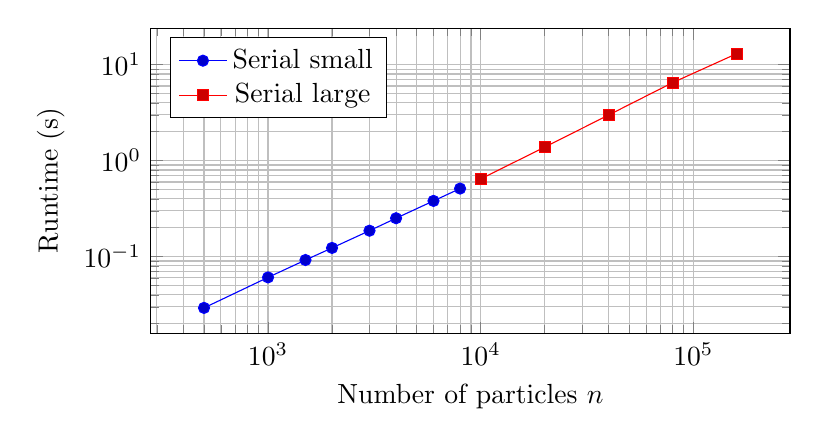
\begin{tikzpicture}
\begin{loglogaxis}[
  width=0.8\linewidth,
  height=0.45\linewidth,
  xlabel={Number of particles \(n\)},
  ylabel={Runtime (s)},
  grid=both,
  legend style={at={(0.03,0.97)},anchor=north west}
]
\addplot+[mark=*] coordinates {
  (500,0.029217) (1000,0.060744) (1500,0.092168) (2000,0.123194)
  (3000,0.186291) (4000,0.251289) (6000,0.380784) (8000,0.512006)
};
\addlegendentry{Serial small}
\addplot+[mark=square*] coordinates {
  (10000,0.645118) (20000,1.38445) (40000,2.99374) (80000,6.51058) (160000,13.0367)
};
\addlegendentry{Serial large}
\end{loglogaxis}
\end{tikzpicture}
\caption{Serial runtime vs.\ particle count on log-log axes.}
\end{figure}

\section{OpenMP Results}
\subsection{Raw Timing Data}
\begin{table}[h]
\centering
\caption{Strong-scaling runs (fixed \(n=10000\))}
\begin{tabular}{rr}
\toprule
Threads & time (s) \\
\midrule
1 & 0.715636 \\
2 & 0.485142 \\
4 & 0.571316 \\
8 & 0.362603 \\
16 & 0.252419 \\
\bottomrule
\end{tabular}
\end{table}

\begin{table}[h]
\centering
\caption{Weak-scaling runs (problem size grows with thread count)}
\begin{tabular}{rrr}
\toprule
Threads & \(n\) & time (s) \\
\midrule
1 & 10000 & 0.715636 \\
2 & 20000 & 0.982823 \\
4 & 40000 & 2.456700 \\
8 & 80000 & 3.086700 \\
16 & 160000 & 4.496490 \\
\bottomrule
\end{tabular}
\end{table}

\subsection{Speedup and Efficiency}
Using baseline serial \(t_0 = 0.644588\) s:
\begin{table}[h]
\centering
\caption{Strong scaling speedup and efficiency}
\begin{tabular}{rrrr}
\toprule
Threads & time (s) & speedup & efficiency \\
\midrule
1 & 0.715636 & 0.9007 & 0.9007 \\
2 & 0.485142 & 1.3287 & 0.6643 \\
4 & 0.571316 & 1.1283 & 0.2821 \\
8 & 0.362603 & 1.7777 & 0.2222 \\
16 & 0.252419 & 2.5536 & 0.1596 \\
\bottomrule
\end{tabular}
\end{table}

\begin{table}[h]
\centering
\caption{Weak scaling efficiency}
\begin{tabular}{rrrr}
\toprule
Threads & \(n\) & time (s) & efficiency \\
\midrule
1 & 10000 & 0.715636 & 0.9007 \\
2 & 20000 & 0.982823 & 0.6559 \\
4 & 40000 & 2.456700 & 0.2624 \\
8 & 80000 & 3.086700 & 0.2088 \\
16 & 160000 & 4.496490 & 0.1434 \\
\bottomrule
\end{tabular}
\end{table}

\begin{table}[h]
\centering
\caption{Average OpenMP scaling efficiency}
\begin{tabular}{lr}
\toprule
Metric & Value \\
\midrule
Average strong scaling efficiency & 0.4458 \\
Average weak scaling efficiency & 0.4342 \\
\bottomrule
\end{tabular}
\end{table}

\subsection{Scaling Plots}
\begin{figure}[h]
\centering
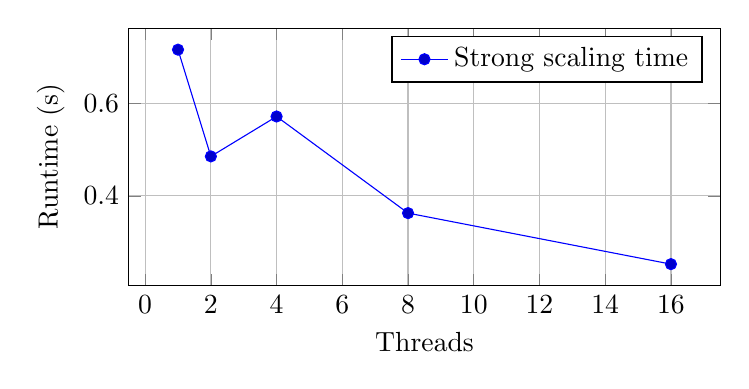
\begin{tikzpicture}
\begin{axis}[
  width=0.75\linewidth,
  height=0.40\linewidth,
  xlabel={Threads},
  ylabel={Runtime (s)},
  grid=both,
  legend pos=north east
]
\addplot+[mark=*] coordinates {(1,0.715636) (2,0.485142) (4,0.571316) (8,0.362603) (16,0.252419)};
\addlegendentry{Strong scaling time}
\end{axis}
\end{tikzpicture}
\caption{OpenMP strong scaling runtime (fixed \(n=10000\)).}
\end{figure}

\begin{figure}[h]
\centering
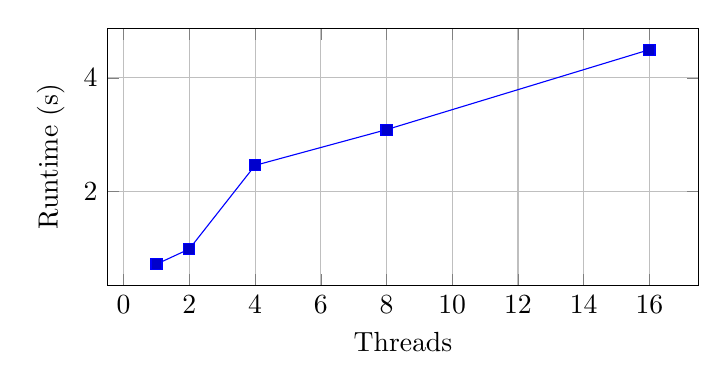
\begin{tikzpicture}
\begin{axis}[
  width=0.75\linewidth,
  height=0.40\linewidth,
  xlabel={Threads},
  ylabel={Runtime (s)},
  grid=both
]
\addplot+[mark=square*] coordinates {(1,0.715636) (2,0.982823) (4,2.456700) (8,3.086700) (16,4.496490)};
\end{axis}
\end{tikzpicture}
\caption{OpenMP weak scaling runtime (\(n\) scales with threads).}
\end{figure}

\begin{figure}[h]
\centering
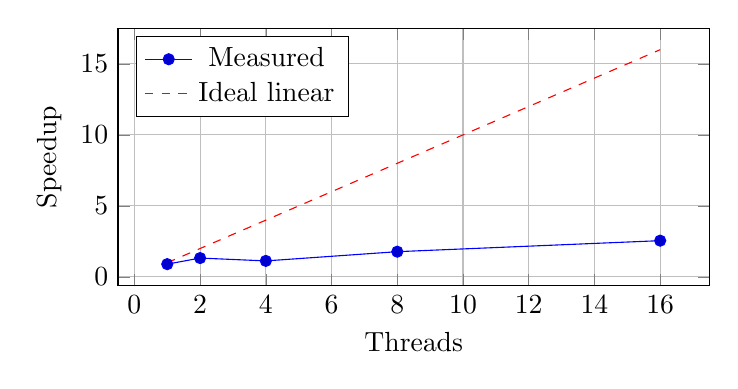
\begin{tikzpicture}
\begin{axis}[
  width=0.75\linewidth,
  height=0.40\linewidth,
  xlabel={Threads},
  ylabel={Speedup},
  grid=both,
  legend pos=north west
]
\addplot+[mark=*] coordinates {(1,0.9007) (2,1.3287) (4,1.1283) (8,1.7777) (16,2.5536)};
\addlegendentry{Measured}
\addplot+[mark=none,dashed] coordinates {(1,1) (2,2) (4,4) (8,8) (16,16)};
\addlegendentry{Ideal linear}
\end{axis}
\end{tikzpicture}
\caption{Strong scaling speedup vs.\ ideal linear speedup.}
\end{figure}

\begin{figure}[h]
\centering
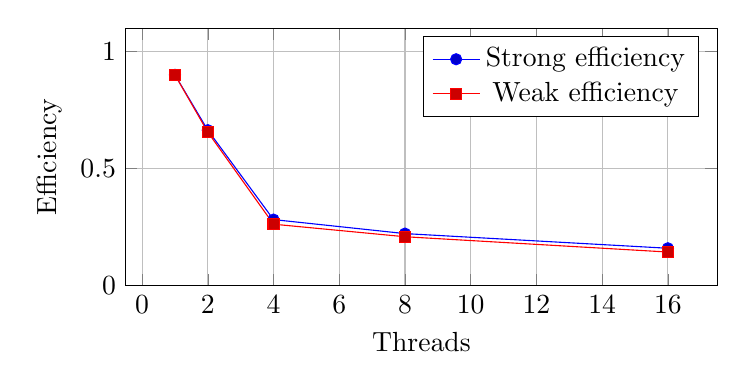
\begin{tikzpicture}
\begin{axis}[
  width=0.75\linewidth,
  height=0.40\linewidth,
  xlabel={Threads},
  ylabel={Efficiency},
  ymin=0, ymax=1.1,
  grid=both,
  legend pos=north east
]
\addplot+[mark=*] coordinates {(1,0.9007) (2,0.6643) (4,0.2821) (8,0.2222) (16,0.1596)};
\addlegendentry{Strong efficiency}
\addplot+[mark=square*] coordinates {(1,0.9007) (2,0.6559) (4,0.2624) (8,0.2088) (16,0.1434)};
\addlegendentry{Weak efficiency}
\end{axis}
\end{tikzpicture}
\caption{Strong and weak scaling efficiency.}
\end{figure}

\section{Discussion}
The serial slope near 1 confirms the expected improvement from all-pairs
\(\mathcal{O}(n^2)\) to cell-list-based \(\mathcal{O}(n)\).

OpenMP scaling improves runtime but remains far from ideal, especially at higher
thread counts. The main limiting factors are:
\begin{itemize}
  \item serial binning phase (\texttt{omp single}) every timestep,
  \item barrier/synchronization overhead between phases,
  \item load imbalance due to non-uniform particle distribution,
  \item memory hierarchy effects and shared-data contention at larger thread counts.
\end{itemize}
For example, at 16 threads the strong-scaling speedup is \(2.55\times\) (ideal
is \(16\times\)), and weak-scaling efficiency at 16 threads is \(0.143\).

\section{Reproducibility and Finalization Notes}
\begin{itemize}
  \item Correctness jobs: \texttt{sbatch job-teach-serial}, \texttt{sbatch job-teach-openmp}
  \item Timing jobs: \texttt{sbatch auto-teach-serial-small}, \texttt{sbatch auto-teach-serial-large},
  \texttt{sbatch auto-teach-omp-small}, \texttt{sbatch auto-teach-omp-large}
\end{itemize}

\subsection{Modified Files and Build Targets}
\begin{itemize}
  \item Core source changes for Part 1: \texttt{serial.cpp}, \texttt{openmp.cpp}.
  \item Build targets used: \texttt{serial}, \texttt{openmp}, \texttt{autograder}.
  \item \texttt{Makefile} was not modified.
\end{itemize}

\end{document}
